\documentclass{article}
\usepackage[utf8]{inputenc}
\usepackage{amsmath, amssymb}
\usepackage{hyperref}
\usepackage{graphicx}
\usepackage{listings}
\usepackage{enumitem}
\usepackage[ruled,vlined]{algorithm2e}
\usepackage{tikz}
\usetikzlibrary{arrows.meta}

\title{Arbitrage Cycle Search Heuristic}
\author{Project Tycho}
\date{\today}

\newcommand{\xin}{x_{\text{in}}}
\newcommand{\yout}{y_{\text{out}}}


\begin{document}

\maketitle

\tableofcontents

\section{Overview}
The Tycho Searcher processes real-time blockchain data and identifies arbitrage opportunities. It receives block updates from a data feed, maintains an up-to-date graph of token exchanges, and applies a modified Bellman-Ford algorithm to detect negative cycles, which correspond to profitable arbitrage paths.

\section{System Architecture}
\begin{itemize}[leftmargin=*, label=--]
    \item \textbf{Tycho Feed:} An asynchronous task receives block updates and token data from an external source, forwarding them to the searcher.
    \item \textbf{Searcher:} Maintains the exchange graph, updates it with new data, and runs the arbitrage detection algorithm.
 \end{itemize}
The code is written in rust. It uses asynchronous channels (\texttt{tokio::sync::mpsc}) to communicate between the feed and the searcher.


\section{Searcher Workflow}
\begin{enumerate}[leftmargin=*, label=\arabic*.]
    \item \textbf{Initialization:} The searcher initializes its graph structures and awaits block updates.
    \item \textbf{Block Update Handling:} On receiving a new block, the searcher updates the graph with the latest exchange rates and liquidity data.
    \item \textbf{Arbitrage Detection:} The searcher runs the modified Bellman-Ford algorithm to find negative cycles, which indicate arbitrage opportunities.
    \item \textbf{Result Export:} Detected opportunities are processed and can be exported or logged for further action.
\end{enumerate}

\section{Modified Bellman-Ford Algorithm}
\subsection{Purpose}
The Bellman-Ford algorithm can detect negative cycles in a weighted graph. It has been adapted for arbitrage search, where the task is to find a cycle with positive profit in the exchange graph. In our adaptation, we consider that the internal state of an Automated Market Maker (AMM) changes after each exchange; therefore, we restrict arbitrage cycles to traverse each AMM at most once.

\subsection{Data Structures}
\begin{itemize}[leftmargin=*, label=--]
    \item \texttt{Graph}: A directed graph where nodes represent tokens and each edge corresponds to an AMM and represents the exchange rates between the corresponding tokens.
    \item \texttt{Edge Weights}: 
Each edge is associated with two functions: $e(\xin)$ and $g(\xin)$. Here, $e(\xin)$ returns the amount of tokens received after the swap, $\yout$, while $g(\xin)$ returns the gas used, which is typically a constant function, since the gas cost is usually independent of $\xin$.

We assume that $e(\xin)$ is a monotone non-decreasing function; that is, increasing the input amount $\xin$ does not decrease the output amount $\yout$. Moreover, the exchange rate $\frac{\yout}{\xin}$ is a monotone non-increasing function of $\xin$.

Each query to $e()$ incurs a computational cost — in practice, this is implemented via a Rust call to \texttt{get\_amount\_out}, which emulates the swap. Both $\xin$ and $\yout$ are stored as large integer values.
\end{itemize}

\begin{figure}
\centering
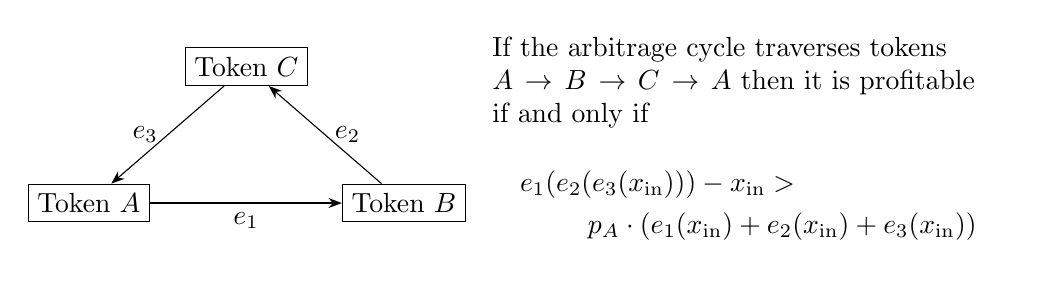
\begin{tikzpicture}[>=Stealth, node distance=2cm]
\node[draw] (A) at (0,0) {Token $A$};
\node[draw] (B) at (4,0) {Token $B$};
\node[draw] (C) at (2,1.732) {Token $C$}; % Equilateral triangle
\draw[->] (A) -- node[below] {$e_1$} (B);
\draw[->] (B) -- node[right] {$e_2$} (C);
\draw[->] (C) -- node[left] {$e_3$} (A);
\node[anchor=west, text width=65mm, align=left] at (5,0.8) {If the arbitrage cycle traverses tokens $A \rightarrow B \rightarrow C \rightarrow A$ then it is profitable if and only if 
\begin{multline*}
e_1(e_2(e_3(\xin))) - \xin > \\ p_A\cdot (e_1(\xin) + e_2(\xin) + e_3(\xin))
\end{multline*}
};
\end{tikzpicture}
\caption{An illustration of arbitrage cycle. $p_A$ is the exchange rate for Token $A$ in ether.}\label{fig:arbcycle}
\end{figure}

Fig.~\ref{fig:arbcycle} illustrates an example of an arbitrage cycle. An arbitrage is defined by a closed path in the (exchange) graph and an input amount $\xin$, which is denominated in the start token. The cycle begins and ends at the same token, referred to as the \emph{start node} or \emph{start token}.

The arbitrage cycle has two key performance metrics:
\begin{enumerate}
\item Gas cost -- the sum of the gas used by each pool along the arbitrage path, including inter-pool transfers,
\item Profit -- the net gain in the amount of the start token.
\end{enumerate}

Since gas is paid in Ether, determining whether an arbitrage is profitable requires knowing the price $p$ of the start token in ETH. If the start token is WETH, then $p = 1$.
 
 For simplicity let's assume $\xin$ is given. Than we can define the following data structure 
 \begin{itemize}[leftmargin=*, label=--]
    \item \texttt{Distances}: 
For each node $v$, we store the maximum attainable output amount $\yout$ (denoted as $d_v$) and the corresponding path $P_v$ from the start node.
 %   To avoid unnecessary data copying, cycles found by the algorithm are stored as reference-counted vectors, reducing memory overhead and improving performance.
\end{itemize}

\subsection{Algorithm Steps}

\begin{algorithm}[tb]
\DontPrintSemicolon 
\caption{Modified Belmman-Ford}\label{alg:MBF}
\KwIn{Directed graph $G$, strat node $s$, amount $\xin$, price $p$}
\nl $d_s=\xin$; $g_s=0$; $d_v=\infty$ and $g_v=0$ for $v\in V \setminus \{s\}$\\
\nl \For{$j \in\{1,\dots, k\}$} {
\nl  \For{ $e_{u \rightarrow v} \in E$ }{
\nl     \If{$d_u\neq \infty$} {
\nl $d',g'=$ \texttt{extend\_path}$(d_u, g_u, P_u, e_{u \rightarrow v})$; \\
\nl     \If{$v=s \And  d'>\xin + p \cdot g'$} {
\nl            \texttt{save\_cycle}$(\xin, P_u + e_{u \rightarrow v})$;
        }
\nl     \If{$v\neq s \And d_v+p\cdot g_v> d'+p\cdot g'$} {
\nl            $d_v =d'$;   $g_v =g'$;       $P_v = P_u + e_{u \rightarrow v}$;
        }
        }
    }
}
\end{algorithm}


Algorithm \ref{alg:MBF} describes the pseudocode of the algorithm. It has following main steps:
\begin{enumerate}[leftmargin=*, label=\arabic*.]
    \item Initialize distances from the source node to all other nodes as infinity, except the source itself (zero and empty path).
    \item For each edge $u \rightarrow v$, if node $u$ has a finite distance (i.e., $d_u \neq \infty$), attempt to extend the path $P_u$ by adding the edge. If this results in more tokens than currently recorded at $d_v$, then update both $d_v$ and $P_v$. See function \texttt{extend\_path} for details.
    
    \item Repeat the previous step for $k$ iterations, where $k$ is the maximum allowed path length.
    %\item After the main loop, check for negative cycles by verifying if any edge can still be relaxed. If so, reconstruct the cycle.
    %\item Store detected cycles as \texttt{Rc<Vec<EdgeIndex>>} to minimize cloning and memory usage.
\end{enumerate}

The function \texttt{extend\_path}$(d_u, g_u, P_u, e_{u \rightarrow v})$ returns the token amount and gas usage resulting from extending path $P_u$ with edge $e_{u \rightarrow v}$. It accounts for the case where the same AMM is traversed multiple times along $P_u + e_{u \rightarrow v}$, updating its internal state after each traversal.

The function \texttt{save\_cycle}$(\xin, P)$ saves a profitable arbitrage cycle with a given amount $\xin$. 

\subsection{Arbitrage search}

Next, we discuss how to search for the optimal input amount $\xin$. We begin by running Algorithm~\ref{alg:MBF} with $p = 0$ and a small initial input, e.g., $\xin = 0.001$, which typically yields multiple arbitrage cycles. For each identified cycle, we apply a black-box optimization method—Golden Section Search (GSS)—to find the optimal $\xin$.

GSS is a derivative-free optimization technique for finding the maximum (or minimum) of a unimodal function over a bounded interval. It is particularly suitable when the function’s analytic form is unknown or too expensive to compute, but function evaluations are available. GSS progressively narrows the interval of interest using the golden ratio, requiring only function values at strategically chosen points. In our setting, GSS is used to identify the input amount $\xin$ that maximizes arbitrage profit along a given cycle.

 
\subsection{Optimizations}

To reduce computation time, we divide the graph into subgraphs and solve the problem independently for each. To compute the subgraphs, we remove the start node $s$ and identify the resulting connected components. Each subgraph is then formed by reintroducing the start node $s$ and connecting it to a component. The algorithm is executed independently within each subgraph.

To further reduce runtime, we implemented the following memory management strategy.
\begin{itemize}[leftmargin=*, label=--]
    \item \textbf{Reference Counting:} By using \texttt{Rc<Vec<EdgeIndex>>}, the algorithm avoids deep cloning of cycle paths, which is especially beneficial when many cycles are detected.
    \item \textbf{Efficient Graph Updates:} Only relevant subgraphs are updated per block, reducing recomputation.
    \item \textbf{BigUint Arithmetic:} Ensures that all calculations are safe from overflow, which is critical for financial computations.
\end{itemize}

%\section{Example: Negative Cycle Detection}
%\begin{lstlisting}[caption=Finding Negative Cycles]
%// Pseudocode for negative cycle detection
%for each node in graph {
%    run bellman_ford from node
%    if negative cycle found {
%        store Rc<Vec<EdgeIndex>> for the cycle
%    }
%}
%\end{lstlisting}
%
%\section{Algorithm Details}
%
%\subsection{High-Level searcher Flow}
%Below is a high-level flowchart of the searcher's main loop:
%
%%\begin{verbatim}
%%Mermaid flowchart (render with mermaid CLI or online)
%%flowchart TD
%%    A["Start: Receive Block Update"] --> B["Update Graph with New Pools/States"]
%%    B --> C["For Each Component"]
%%    C --> D["Run Bellman-Ford from Start Node"]
%%    D --> E["Relax Edges for N Iterations"]
%%    E --> F["Detect Negative Cycles"]
%%    F --> G["For Each Cycle"]
%%    G --> H["Optimize Input Amount (Golden Section Search)"]
%%    H --> I{"Profit > 0?"}
%%    I -- "Yes" --> J["Log/Export Arbitrage"]
%%    I -- "No" --> K["Skip"]
%%    J --> L["Wait for Next Block"]
%%    K --> L
%%    L --> A
%%\end{verbatim}
%
%\subsection{Bellman-Ford Relaxation and Negative Cycle Detection}
%
%%\begin{verbatim}
%%Mermaid flowchart (render with mermaid CLI or online)
%%flowchart TD
%%    subgraph BellmanFord["Bellman-Ford Relaxation Loop"]
%%        B1["Initialize distances: ∞, source=0"]
%%        B2["Repeat for |V|-1 iterations:"]
%%        B3["  For each edge (u,v):"]
%%        B4["    If d[v] > d[u] + w(u,v):"]
%%        B5["      d[v] = d[u] + w(u,v)"]
%%        B6["      pred[v] = u"]
%%        B2 --> B3 --> B4 --> B5 --> B6
%%    end
%%    B1 --> B2
%%    B6 --> C["Check for negative cycles"]
%%    C --> D{"Any edge can still be relaxed?"}
%%    D -- "Yes" --> E["Reconstruct cycle using pred[]"]
%%    D -- "No" --> F["No negative cycle"]
%%    E --> G["Store cycle as Rc<Vec<EdgeIndex>>"]
%%    F --> H["Done"]
%%    G --> H
%%\end{verbatim}
%
%\subsection{Component Interaction Sequence}
%
%\begin{verbatim}
%%% Mermaid sequence diagram (render with mermaid CLI or online)
%sequenceDiagram
%    participant S as searcher
%    participant G as Graph
%    participant B as BellmanFord
%    participant O as Optimizer
%    S->>G: Update with new block
%    S->>B: Run Bellman-Ford
%    B->>G: Relax edges
%    B->>B: Repeat for N iterations
%    B->>G: Check for negative cycles
%    B-->>S: Return cycles
%    S->>O: For each cycle, optimize input amount
%    O-->>S: Return best amount, profit
%    S->>S: If profit > 0, log/export arbitrage
%    S->>S: Wait for next block
%\end{verbatim}
%
%\subsection{Pseudo-code}
%
%\textbf{Main searcher Loop:}
%\begin{lstlisting}[]
%loop {
%    receive block update;
%    update graph with new pools/states;
%    for each component in graph {
%        run Bellman-Ford from start node;
%        for each negative cycle found {
%            optimize input amount (golden section search);
%            if profit > 0 {
%                log/export arbitrage;
%            }
%        }
%    }
%}
%\end{lstlisting}
%
%\textbf{Bellman-Ford Relaxation:}
%
%
%\textbf{Negative Cycle Detection:}
%\begin{lstlisting}[]
%for each edge (u, v) {
%    if d[v] > d[u] + w(u, v) {
%        // Negative cycle found
%        reconstruct cycle using pred[];
%        store cycle as Rc<Vec<EdgeIndex>>;
%    }
%}
%\end{lstlisting}
%
%\textbf{Profit Optimization (Golden Section Search):}
%\begin{lstlisting}[]
%fn optimize_cycle_gss(cycle, graph, source, min, max, tol, max_iter, gas_price) {
%    // Search for input amount that maximizes profit
%    let (best_x, best_profit) = golden_section_search(min, max, tol, max_iter, |x| {
%        let profit = simulate_cycle_profit(cycle, x, graph, source, gas_price);
%        return profit;
%    });
%    return (best_x, best_profit);
%}
%\end{lstlisting}

\subsection{Edge Cases:}
\begin{itemize}
    \item Cycles are only considered if they start and end at the designated start token (e.g., WETH).
    \item Reference-counted vectors (\texttt{Rc<Vec<EdgeIndex>>}) are used to avoid unnecessary cloning.
    \item The algorithm skips cycles that revisit nodes to avoid infinite loops.
    \item Profit calculation includes gas costs, and only cycles with net positive profit are exported.
    \item The golden section search adapts the input range if invalid points are encountered.
\end{itemize}

\section{Conclusion}
The Tycho Searcher combines real-time data processing with efficient graph algorithms to detect arbitrage opportunities in decentralized exchanges. The use of optimized data structures, such as reference-counted vectors and big integer arithmetic, ensures both performance and correctness.

\end{document} 